\section{Planificación de las actividades}

Aquí se define el modelo de ciclo de vida de la ontología. El ciclo de vida que se adapta a los escenarios elegidos es el Modelo de Cascada de 6 fases, debido a que serán necesarias las fases de reuso tanto de recursos ontológicos como no-ontológicos, reingeniería, y diseño para la implementación. En la Figura \ref{img:secuenciaDeDesarrollo} se muestra el modelo de ciclo de vida a seguir. Se decidió utilizar el Modelo de Ciclo de Vida Cascada ya que el alcance de la ontología es bien delimitado y el tiempo acotado.

\begin{figure}[ht!]
    \centering
    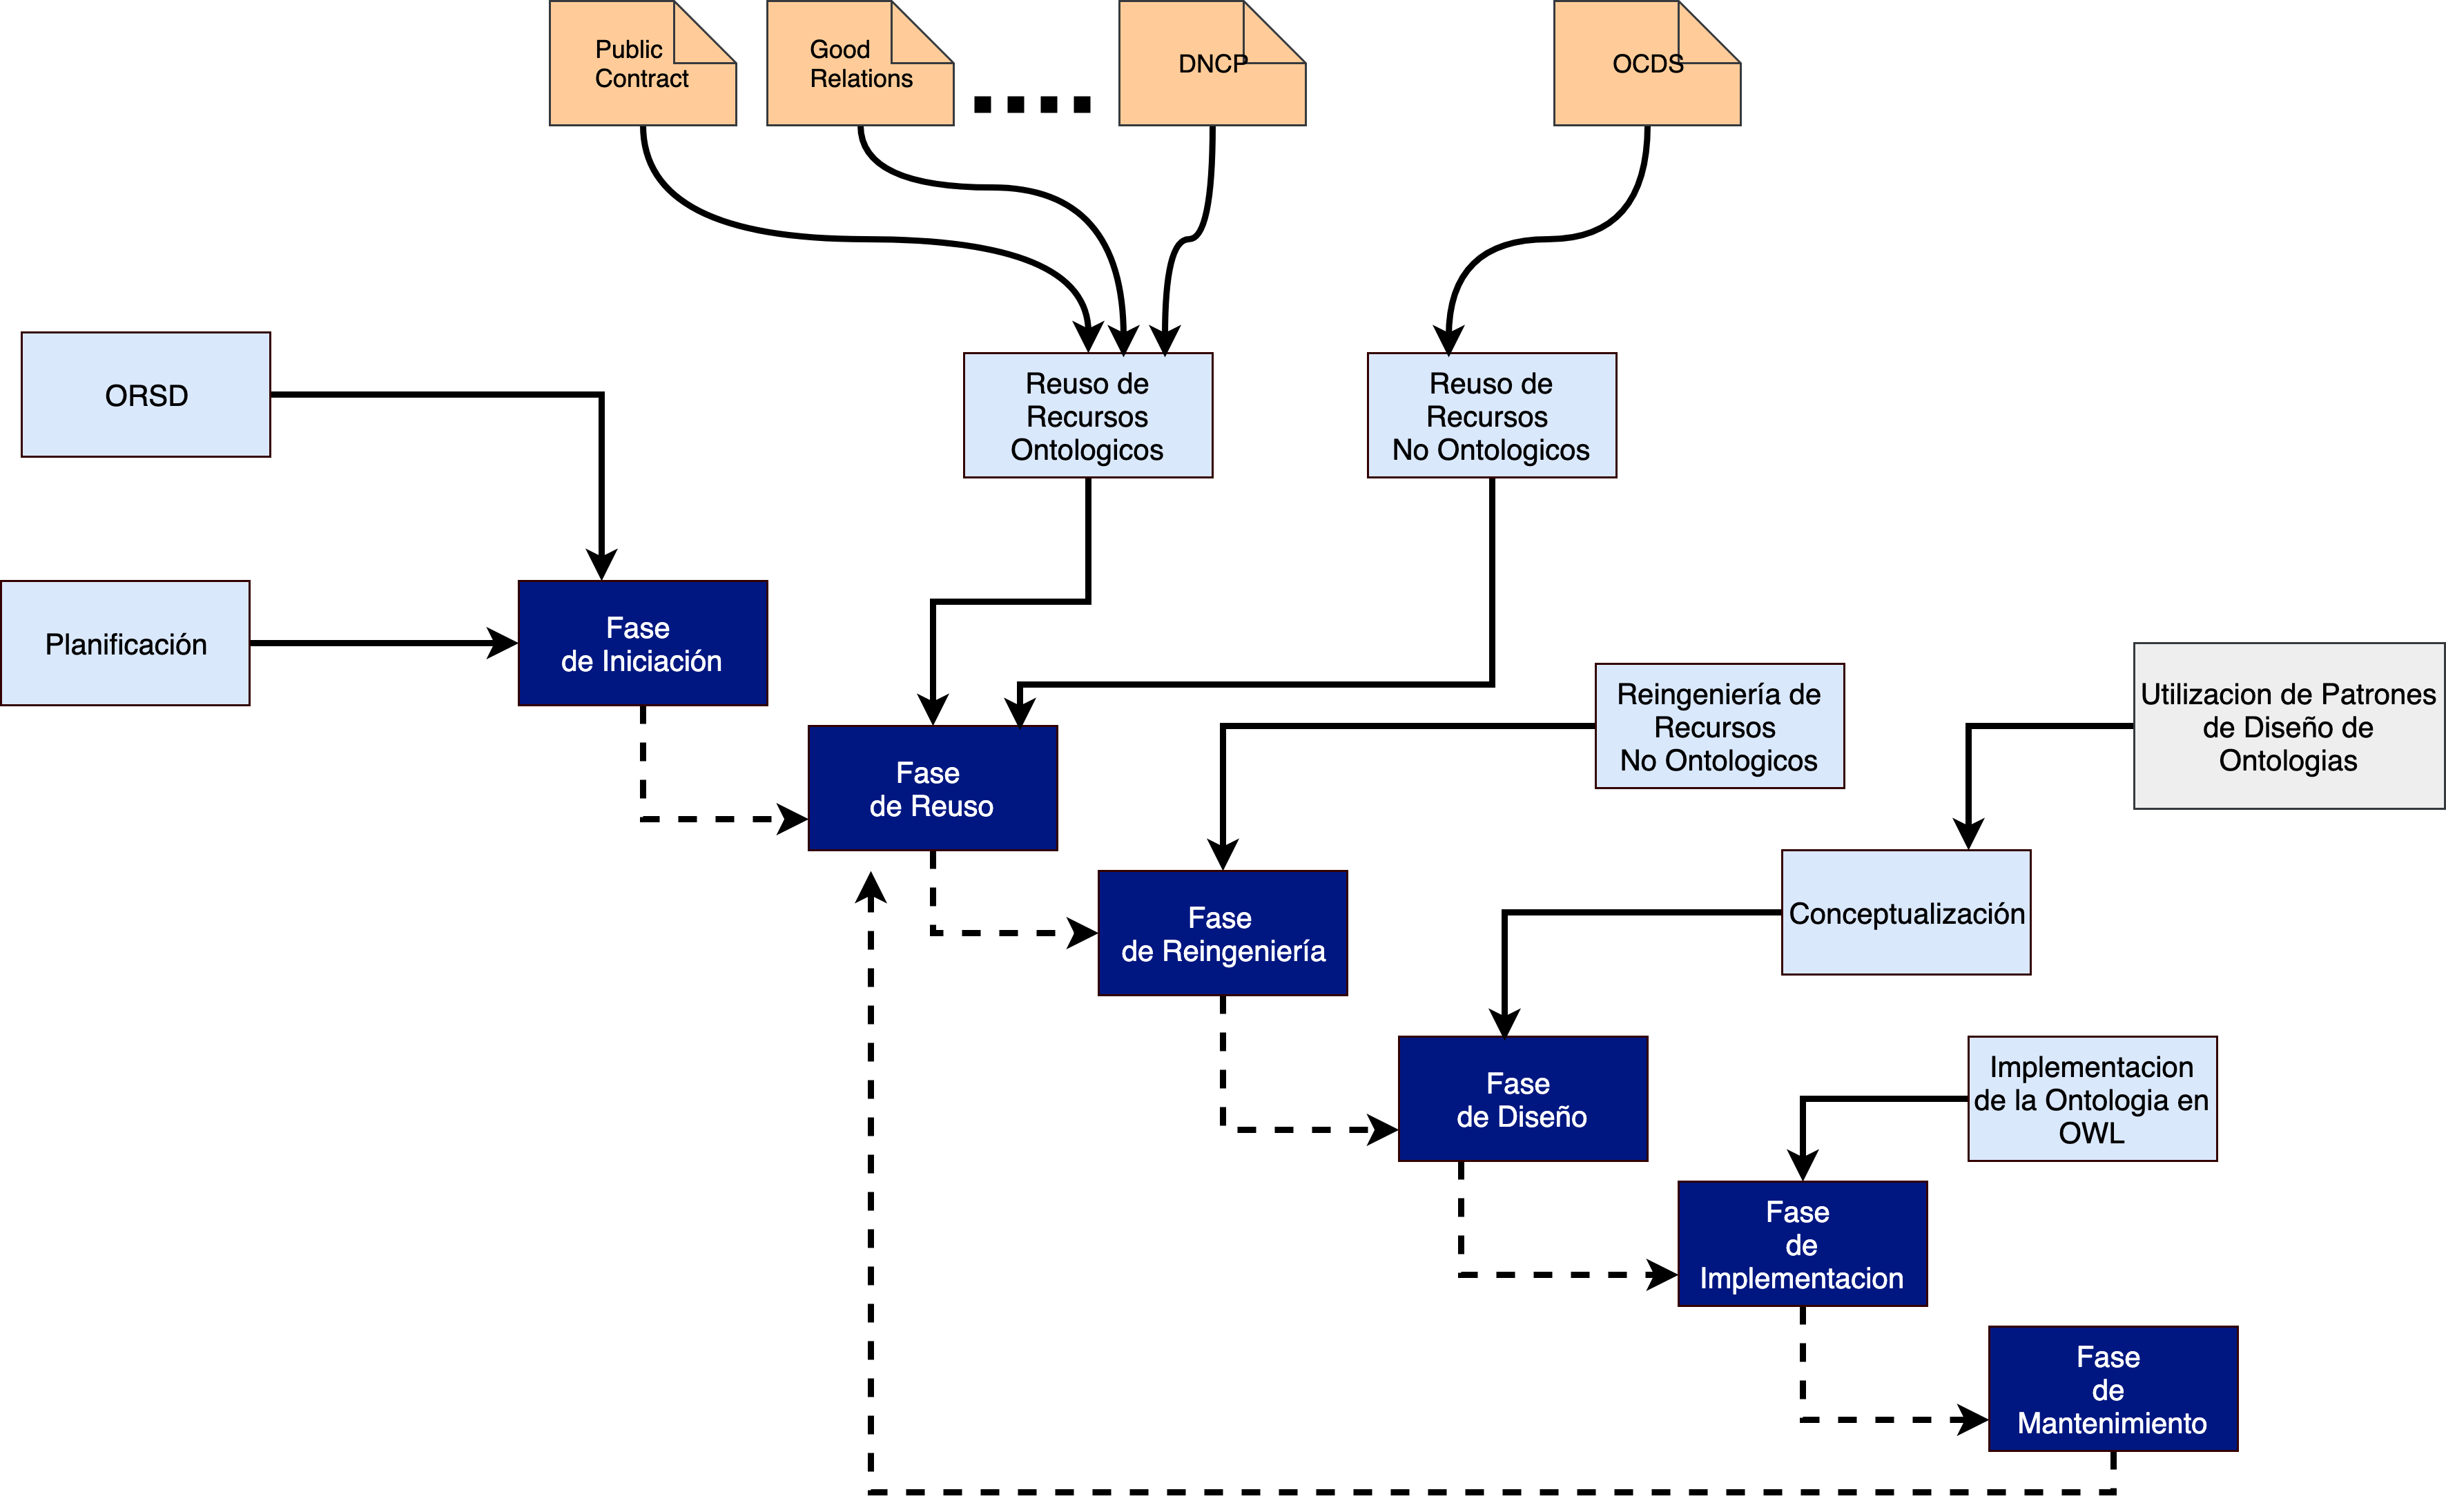
\includegraphics[width=150mm]{figuras/Diagramas-GraficodeSecuenciasDesarrollo.png}
    \caption{Modelo de Ciclo de Vida de desarrollo de la ontología.}
    \label{img:secuenciaDeDesarrollo}
\end{figure}

A continuación se citan las actividades divididas en las fases del ciclo de vida a desarrollarse según la metodología NeOn:
\begin{enumerate}
\item Fase 1: Iniciación
    \begin{enumerate}
    \item Especificación de Requerimientos Ontológicos (ORSD). Aquí se define el propósito de la ontología, su alcance, el lenguaje de implementación, el grupo objetivo, los potenciales usos de la ontología, los requerimientos funcionales y no funcionales, y un pre-glosario de términos.

    \item Planificación. Según lo expuesto en la Tabla \ref{escenarios vs modelo} se elige el modelo de ciclo de vida de 6 fases en cascada, debido a que serán necesarias las fases de reuso tanto de recursos ontológicos como no-ontológicos, reingeniería, y diseño para la implementación.
 
    \end{enumerate}
\item Fase 2: Reuso
    \begin{enumerate}
    \item Reuso de Recursos  no-ontológicos. Los recursos no-ontológicos (NOR) representan recursos de conocimiento cuya semántica no fue formalizada por una ontología. Estos NORs contienen conocimientos de un dominio en particular y representan algún grado de consenso colectivo.

    \item Reuso de Recursos Ontológicos. A fin de no redoblar esfuerzos y con la intención de integrar esta nueva ontología con otras, se procede al reuso de recursos ontológicos. En esta actividad se procedió a la búsqueda, evaluación y selección de las ontologías a reusar.
    \end{enumerate}
\item Fase 3: Reingeniería
\begin{enumerate}
\item Reingeniería de Recursos No-Ontológicos. En esta actividad se analizan posibles patrones de diseño a la hora de la implementación, así como una metodología para transformar la semántica incluida en el OCDS.

\end{enumerate}
\item Fase 4: Diseño
\begin{enumerate}
\item Conceptualización de la Ontología. En esta actividad se identifica el esquema de recursos así como también los componentes conceptuales y sus relaciones. Además, se crea un modelo conceptual dividido por bloques de conceptos relacionados. El conocimiento se expresa mediante representaciones primitivas de conceptos y relaciones entre conceptos. A continuación se representa la conceptualización teniendo como base el OCDS. 

\end{enumerate}
\item Fase 5: Implementación. En esta actividad se procede al desarrollo de la ontología utilizando la herramienta Protégé, el lenguaje utilizado fue OWL, un estándar internacional para codificar e intercambiar ontologías diseñada para la Web Semántica. 

\item Fase 6: Mantenimiento. Por último se procede a la fase del mantenimiento, que consiste en corregir o aumentar los conceptos y restricciones de la ontología para que responda a la preguntas y la detección y corrección de errores de la misma. 		

\end{enumerate}
Una vez terminada la planificación se procede al desarrollo de cada una de las demás actividades siguiendo el orden de las fases. La explicación de cada una de las actividades se describen a continuación en este documento.
